\section{Introduction}
\label{sec:introduction}

% state the learning objective 
The objective of this laboratory assignment is to study a circuit containing a
DC voltage source $V_I$ and a DC current source connected to seven resistors $R_{1-7}$, a linear voltage-controlled current source and a  linear current-controlled voltage source. The circuit can be seen if Figure~\ref{fig:rc}.\\


In Section~\ref{sec:analysis}, it was used the mesh and node analysis methods to solve the circuit. In Section~\ref{sec:simulation}, the circuit is analysed by
simulation, and the results are compared to the theoretical results obtained in
Section~\ref{sec:analysis}. The conclusions of this study are outlined in
Section~\ref{sec:conclusion}.

\begin{figure}[h] \centering
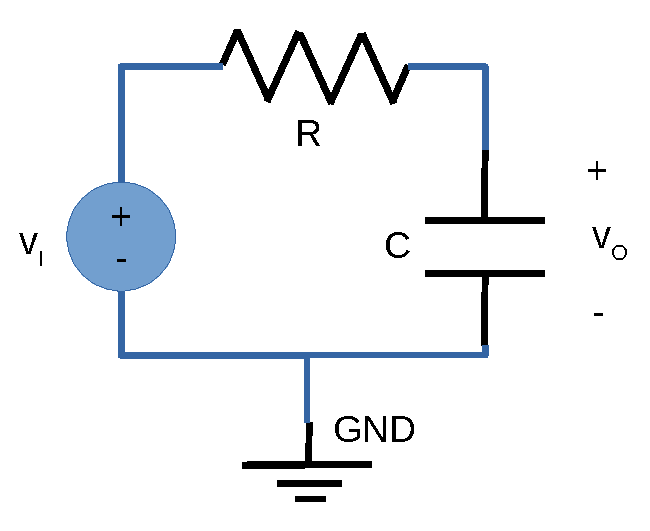
\includegraphics[width=0.4\linewidth]{rc.pdf}
\caption{Voltage driven serial RC circuit.}
\label{fig:rc}
\end{figure}

